\documentclass[
a4paper,   
headsepline, 
fleqn,     
12pt
]{scrartcl}

%%% ngerman: language set to new-german
\usepackage{ngerman}
\usepackage[latin1]{inputenc}
\usepackage[T1]{fontenc}
\usepackage{ae,aecompl}

%%% Graphic stuff
\usepackage{graphicx}
\usepackage{amsmath,amssymb,amstext}
\usepackage{units}
\usepackage{scrpage2}

\setlength{\parindent}{0em} 

\newcommand{\mygraphics}[3]{
  \begin{center}
    \includegraphics[width=#1, keepaspectratio=true]{#2} \\
    \textbf{#3}
  \end{center}
}

%%%      footer - middle: page number
\pagestyle{scrheadings}

%%% heading - left
 \ihead[]{Kevin Wallis}

%%% heading - right
 \ohead[]{Aufgabe 0}

\begin{document}

 \pagenumbering{roman} %% small roman page numbers
 \pagenumbering{arabic} 


\subsection*{Berechnen des nichttrivialen Systemgleichgewichts}
\label{sec:Systemgleichgewicht}

$0=r*(1-\frac{u}{U_k})*u-\frac{w*u*v}{u+K_u}$ \\
$0=s*(1-J*\frac{v}{u})*v$ \\
\textbf{Vorgegebene Werte:} $r=2.5;U_k=300;w=5;k_U=50;s=0.225;J=2$

\begin{enumerate}
\item Umstellen der zweiten Gleichung auf $v$, es gibt zwei L�sungen ($v=0$ und $v=\frac{u}{J}$), die nichttriviale wird genommen: $v=\frac{u}{J}$
\item Die zweite Gleichung kann in die erste eingesetzt und auf folgende Gleichung umgeformt werden: \\ 
$0=u^2+u*k_U-U_k*K_u$ \\
$0=u^2+u*50-15000$ \\
Es gibt zwei L�sungen: $u_1=100$ und $u_2=-150$ \\
Da es keinen negativen Beutebestand geben kann, kommt nur $u_1$ in Frage, daraus ergibt sich $v=50$
\end{enumerate}

Somit ist die nichttriviale L�sung $u=100$ und $v=50$. Die berechneten Werte wurden anhand einer Simulation getestet und f�r passend befunden. Eine Grafik des Simulationsergebnisses kann aus dem Anhang entnommen werden.

\subsection*{Steady State Typ bei den vorgegebenen Anfangswerten}
$u^{(0)}=50;v^{(0)}=60$

Periodisch oszillierender Steady State.

\begin{figure}[h]
  \centering
  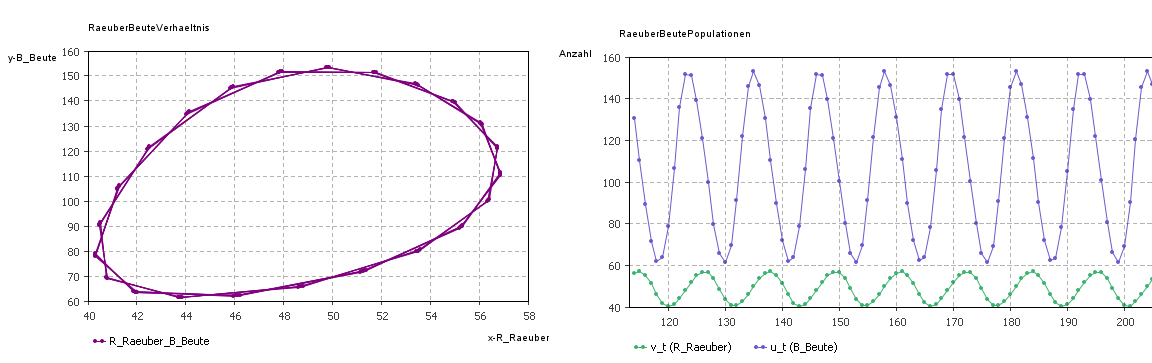
\includegraphics[width=0.6\textwidth]{./images/SteadyState}
  \caption[Steady state: Simulation]{Simulation des Steady states}
  \label{fig:SteadyState}
\end{figure}

\subsection*{Untersuchung der Stabilit�t des Steady States}
Es gibt mehrere M�glichkeiten der Parametervariation, welche anhand einer Simulation �berpr�ft werden m�ssen. Dazu z�hlen das Erh�hen von $v$ bzw. $u$, das erniedrigen der beiden Parameter sowie die beiden Parameter gleichzeitig ver�ndern. \\

Der Steady State ist ein Attraktor, d.h. selbst bei Ver�nderungen wird wieder zum gleichen Station�rzustand zur�ckgekehrt. In Abbildung \ref{fig:SteadyState} ist der Steady State, welcher im wieder eingenommen wird, ersichtlich. 


\appendix  
\bibliographystyle{plain}
\bibliography{projekt.bib}

\end{document}